\section{Auswertung}
\label{sec:Auswertung}

\begin{figure}
  \centering
  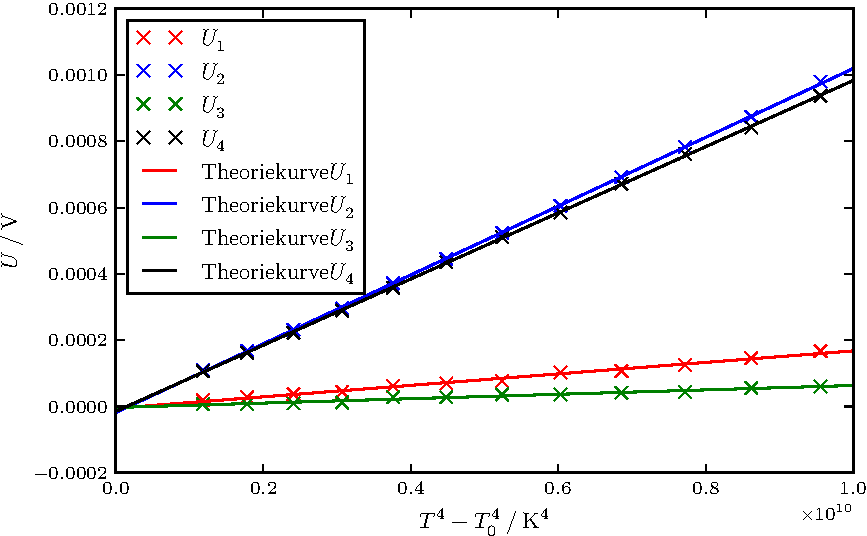
\includegraphics{plot.pdf}
  \caption{Plot.}
  \label{fig:plot}
\end{figure}

\begin{table}
  \centering
  \caption{Beispieltabelle}
  \label{tab:tabelle_beispiel}
  \sisetup{table-format=1.2}
  \begin{tabular}{c c}
    \toprule
    {$a [\si{\second}]$} & {$b [\si{\kelvin}]$}\\
    \midrule
    1.0000  & 11.00 \\
2.0000  & 12.00 \\
3.0000  & 13.00 \\
4.0000  & 14.00 \\
5.0000  & 15.00 \\
6.0000  & 16.00 \\
7.0000  & 17.00 \\
8.0000  & 18.00 \\
9.0000  & 19.00 \\
10.0000 & 20.00 \\

    \bottomrule
  \end{tabular}
\end{table}

Es ergibt sich
\begin{align}
  a &= (0 \pm 0) ~ \si{\joule\per\kelvin\per\gram}
 \\
\end{align}
